\chapter{INTRODUCTION}

\section{Introduction}

The RS274/NGC standard interpreter is a software system that reads numerical control code in the NGC dialect of the RS274 numerical control language and produces calls to a set of canonical machining functions. The output of the interpreter can be used to drive Computerized Numerical Control (CNC) machines with three to six axes. \\

There are many merits of parametric interpolation over the traditional linear and circular interpolation, specifically in terms of model representation, feedrate smoothness and application range. One of the major difficulties of parametric interpolation is the feedrate determination that satisfies geometrical constraints and kinematical characteristics of different CNC machine tools.\\

A majority of CNC systems today supports parametric interpolation because of its various advantages over traditional linear and circular interpolations. The linear interpolator (G01) and the circular interpolator (G02, G03) are the only two interpolators defined in the RS274 standard. References: \cite{Suh-etal:2008}, and \cite{Kramer-etal:2000}. This standard does not have the NURBS interpolator yet that can handle parametric curves and surfaces.\\

Parametric interpolation is conducted as a point-to-point (PTP) movement in a CNC machine. At the end of each motion it is important that the positional accuracy of the tool relative to the workpiece is achieved, that is, within a specified error tolerance ($\epsilon$). At the end of each motion, the tool performs its required task after which the next motion begins and the cycle repeats until all machining is completed. Reference: \cite{Zhong-etal:2018}.

\clearpage
\pagebreak 

In CNC machine operation, the function of interpolation is to generate coordinated movements to drive the separate axis-of-motions in order to achieve the desired path of the CNC cutting tool relative to the workpiece. Essentially, interpolation generates commands that move motor drives to follow the desired path or trajectory to produce the physical part that is being machined.\\

Generally, the contour error is a measure of how close the actual tool path is to the desired tool path. For a two-dimensional parametric curve, the point-to-point movement turns the contour error (positional accuracy) to become the chord-error $\epsilon$. This is the error between two interpolated points for the parametric curve. Reference: \cite{Sun-etal:2018}

\section{Problem statement}

\begin{figure}
	\caption{Concept of Chord-error $\epsilon$, Feedrate F, and Interpolation time T } Source: \cite{Nguyen-etal:2017}
	\label{chap1-Chord-error-image.png}
	\centering
	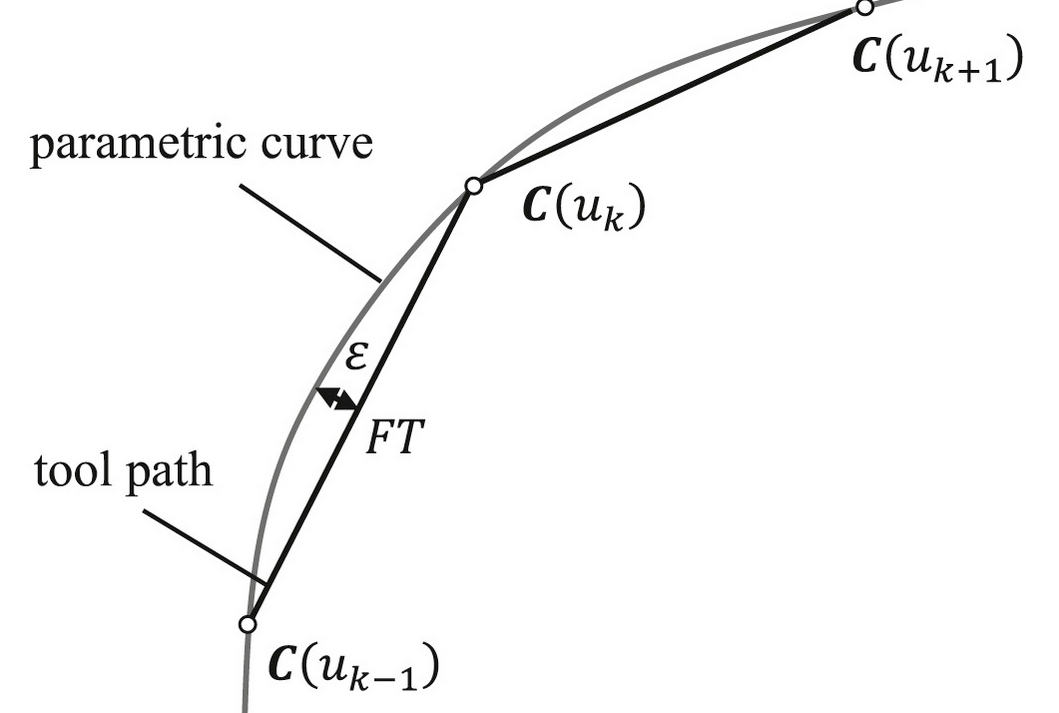
\includegraphics[width=0.80\textwidth]{Images/Chap3/Chord-error-image.png} 
\end{figure}


Generally, for a specific curve path, an increase in feedrate F, will decrease the total number of interpolated points but will increase the chord length (FT), of each arc segment, thereby increasing the chord-error $\epsilon$. \\

On the other hand, a decrease in feedrate will increase the total interpolated points and reduce the chord-error but will cause the overall machining operation to be slow and time consuming. Thus, there is an interplay between chord-error $\epsilon$, and machine feedrate F. The problem is how to find an optimum balance. \\

This work proposed a solution by developing a realtime parametric curve interpolation algorithm that constrains both the feedrate and chord-error simultaneously. It was developed and tested for ten(10) different 2-dimensional parametric curves. \\ 

The curves were selected based on complex shape characteristics like closed loop curves, open ended curves, symmetric or non-symmetric about the x-axis and y-axis. Some curves have sharp, concave or convex turns including cusps. In addition, the x and y dimensions, that is, their overall sizes vary among the different curves. These are some of the geometrical constraints of the algorithm.\\ 

The dynamical and kinematical constraints cover specific CNC machine characteristics like the maximum and minimum allowable machine velocities and accelerations for the different axes of motion, the user specified command feedrate, the jerks and jitter that in combination affects the smooth operation of the machine.  References: \cite{Yeh:2019}, \cite{Yu-etal:2020}, and \cite{Rob:2022}.


\section{Motivation}

Ever since the author was a child, there were always fascinations with regards to moving things and objects, both animated and non-animated. If growth is considered a movement, then humans, animals and plants grow. Whereas the growth of humans and animals are in years, the "growth movements" of vegetation, for example, trees, shrubs and vegetables can be in days, weeks, months and in years, that is, on very different time scales. Humans and animals can move instantly, by choice or instincts. \\

Inanimate objects, though inherently non moving, can be made to move. Manufacturing robots, vehicles, satellites, spaceships, underwater submarines, drones, missiles and Computerized Numerical Control (CNC) machines, are examples of inanimate objects that can move or move others, with the help of motors, hydraulics, electrical, chemical, wind, wave power, and so on. These inanimate objects can move guided or autonomously by some control system, typically but not necessarily using software.\\ 

For example, fighter bombers during the Second World War (early to mid 1940s) were manually controlled using hydraulics by human pilots because there was no software. Thousands of years ago, the ancient Egyptian system for flood and irrigation control of the Nile river uses water wheels and water mills. Software and computing machines were not invented yet so there was no software to use at that time.\\ 

The Apollo Control and Guidance System (ACGS developed by MIT) was a crude combination of basic software, hardware and electronics. The system successfully sent humans to the moon, landed and returned them to earth safely in the late 1960s. This is a very significant landmark in human history.\\ 

In particular, CNC machines for example, move electric motors for cutting drills (milling or engraving), lasers and high pressure water jets to cut materials and produce diverse and useful products for humans. Today, the use of software to control movements of some systems is almost ubiquitous.\\ 

With the author's having access to a bare-bones prototype CNC machine, the interest grew into the complex world of animating non-animated objects. This led to the current endeavor in CNC machine and its control software, the interpolation program. \\

Basically, in order to produce the physical part that is being machined, the interpolation program generates commands that move motor drives step-by-step and point-to-point to follow the desired path or trajectory. \\

Moving inanimate objects is not limited to just cutting things like in the CNC machine. It is also about robots moving around, avoiding obstacles, and performing actions beyond what humans can do, in the air or underwater, in guided or autonomous modes. The possibilities are endless.

\section{Brief description of this thesis}   

\noindent 
The work in this thesis is about mechatronics and system design. The topic in this work covers five(5) major themes described as follows.

\begin{enumerate}
	\item Parametric curve - a special mathematical representation of a path trajectory 
	
	\item Interpolation - the activity of determining the successive "next-points" in following the specified path trajectory
	
	\item Chord-error - the error between the actual "moved" position and its required position according to the specified path
	
	\item Feedrate - the actual speed of motion along the path.
	
	\item Realtime - the current time in execution by point-to-point moves along the path.
	
\end{enumerate}

\noindent
From the above themes, this work is appropriately titled \textbf{"Realtime interpolation of parametric curves with chord-error and feedrate constraints."} \\

\noindent
The next section presents an example of the expected results of this thesis.

\clearpage
\pagebreak

\section{About end results of this thesis} \label{sec-About end results of this thesis}

\begin{figure}
	\caption  {Butterfly Perspective View 3D in LinuxCNC-Axis}
	\label{img-Chap1-Butterfly-Perspective-View-3D-from-LinuxCNC-Axis.png}
	\centering
\framebox{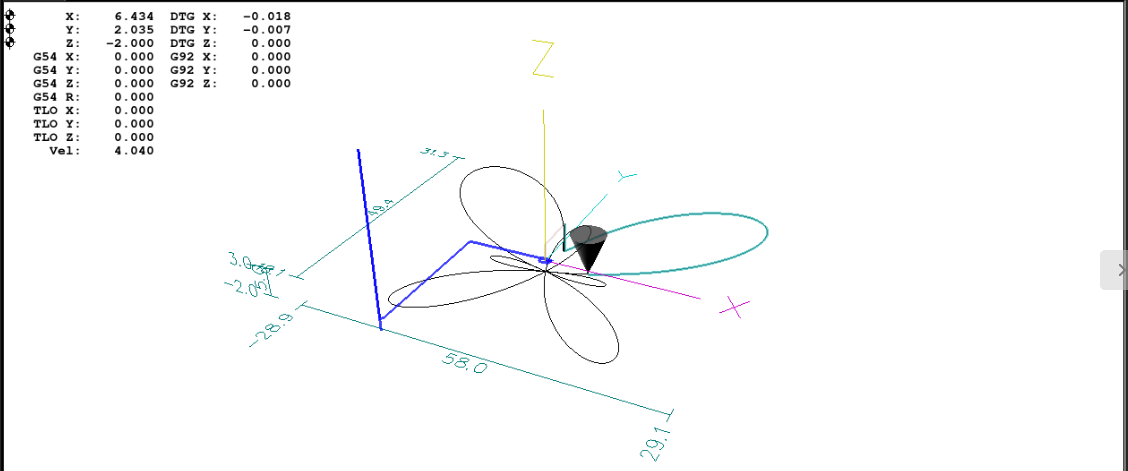
\includegraphics[width=1.00\textwidth]{Chap1/images/img-Chap1-Butterfly-Perspective-View-3D-from-LinuxCNC-Axis.png} }
\end{figure}	

The end results of this thesis can be described as follows. The work in this thesis is about generating a single interpolation algorithm that is successfully applied to ten(10) different parametric curves of various shapes and dimensions. The above figure shows a real live execution of the Butterfly parametric curve (one of the ten curves), by the algorithm developed in this work. \\

The job of the interpolation algorithm is to generate successive points along the curve trajectory so that the CNC cutting tool (laser cutter) illustrated by the cone in the figure follows the path accurately. The curve begins at parameter u = 0.00 (starting point), increasing in steps until u = 1.00 (ending point), as the entire Butterfly curve is being followed, that is, from start to finish. \\

The algorithm uses the second-order Taylor's approximation to calculate the steps (u-next) in parameter u, and at the same time constrains both the chord-error (deviation from the true curve path) to below a set error tolerance (1E-6 mm), and the running feedrate to be very close but below the feedrate limit throughout the full curve path. \\

The feedrate limit at every parameter u point is calculated by the algorithm based on geometrical, dynamical and kinematical constraints. The constraints comprise 4 different components: user set Feedrate Command FC, minimum and maximum CNC machine axial velocities, minimum and maximum CNC machine axial accelerations, and the geometric factors of the curve path like bends and sharp turns. \\

\clearpage
\pagebreak

The main objective of the algorithm execution is to ensure that the resulting running feedrate (speed motion of the cutting tool) is smooth and continuous, and not exceeding the feedrate limit throughout the full curve path. Note that the feedrate limit varies with u, and thus, the running feedrate also varies, for example, when negotiating curves and sharp bends. The algorithm accomplishes the tool motion strictly without violating both the chord-error and running feedrate constraints. \\

Since the smoothness of running feedrate is critical to the success of the algorithm, any acceleration jitters (rapid acceleration fluctuations) will result in jerky machine feedrates. The algorithm execution was able to completely avoid this situation. 

%% =============================================
%% \clearpage
%% \pagebreak

\section{Scope of work for this thesis}

The scope of work for this thesis can be described as follows:

\begin{enumerate}
	\item Selection of ten(10) different parametric curves and their equations, each curve with varying features, shapes and dimensions.
	
	\item Setting up the feedrate (velocity) constraining dynamic equations for allowable CNC machine parameters like the maximum and minimum axial velocities, and maximum and minimum axial accelerations.  
	
	\item Setting up the chord-error constraining equations involving geometric and kinematic properties of the ten(10) different parametric curves.
	
	\item Development of a realtime algorithm that generates interpolated points which traverses each curve, such that the chord-error and feedrate at all points are simultaneously constrained.  
	
	\item Execution of reports that show the interpolation algorithm performs correctly as designed, generating interpolated points and feedrates that are smooth and continuous for all ten(10) parametric curves selected. 
	
	\item In addition, the reports on algorithm implementation show that the absolute constraints on chord-error and feedrate are not violated throughout the full trajectory of each curve. 
	
	\item The execution of the algorithm on all ten(10) curves also show that acceleration jitters do not occur, and the acceleration is always maintained between the designed maximum and minimum limit.   
	
	\item The algorithm also generates RS274/NGC G-Code file for validation and verification on the CNC machine running the LinuxCNC-Axis control application.
	
	\item For the performance assessment of the developed algorithm, four different metrics were created. The four metrics are:
	
	\begin{itemize}
		\item SCE/TIP, that is the ratio of total sum-chord-error divided by the total number of interpolated points.
		
		\item SCE/SCL, that is the ratio of total sum-chord-error divided by the total sum-chord-length.
		
		\item SAA/SCL, that is the ratio of the sum-arc-areas divided by the total sum-chord-length.
		
		\item 100(SAL-SCL)/SAL, that is the ratio of the difference between the sum-arc-length and the sum-chord-length, divided by the sum-arc length and multiplied by 100 to represent it in percentage form.
		
	\end{itemize}
	
	\item The results in the main document of this thesis discuss the full outputs of the Teardrop curve resulting from the algorithm execution. The outputs for the rest of the nine(9) selected curves are provided in their respective appendices.	
	
\end{enumerate}




%% =========================================
\clearpage
\pagebreak

\section{Organization of this thesis document}

Chapter 1 Introduction, covers the basic ideas on parametric interpolation, Computerized Numerical Control (CNC) machines, the G-code standards for these CNC machines, chord-error and machine feedrates associated with CNC machining operations. The introduction also includes the problem statement and the motivations that led to this work. Finally, the organization structure of this thesis is documented.\\ 

Chapter 2 Literature Review, involves the topics on mathematical parametric representation of curves and surfaces in NURBS, the general ideas on $C^{N}$ continuity of curves and surfaces and, the advantages of parametric representations. This chapter also includes the concepts of interpolation of parameteric curves. It is followed by a literature review of published sources for previous works involving interpolation of parametric curves and surfaces. At the end of this chapter, the ideas of NURBS and its relationship to CNC G-code programming languages were discussed.\\

Chapter 3 Methodology, begins with describing the processing steps involved in parametric curve interpolation, and include the characteristics and presentation of mathematical equations for the ten(10) parametric curves selected for this work. It is followed by the discussion on chord-error (epsilon) concepts, the chord-error minimization, feedrate maximization, and the proposed combined chord-error and feedrate constraints to be enforced simultaneously. Next, the criteria of convergence is stated in the brief algorithm design for this work. \\ 

Chapter 3 continues with the mathematical derivations of equations to be computed in the algorithm. This includes equations for the radius of curvature ($rho$), chord-error ($epsilon$), current feedrate ($curr\_frate$). The derivations of the first and second order iterative Taylor's expansion followed. This chapter then continues with the calculations for the next interpolation point. The discussions and equations for the various feedrate limits ($frate\_limit$), consisting of the combined dynamical and geometrical constraints were presented. The main program for the interpolation was described through a flowchart. The equations and flowcharts for the rising and falling of feedrates using the sigmoid S-curves were derived, discussed and presented. Chapter 3 ends with the presentation of a flowchart for the balance of chord-error and feedrate combined constraints. \\

Chapter 4 Results, presents the final outcomes of the entire work for this thesis. Out of the ten(10) parametric curves studied in this work, the full results of only one(1) of those curves, for illustration, are presented in the main document. The full results for the rest rest of the curves (about 20 pages per curve) are provided in the respective appendices. The full results for the rest of the curves can be compiled into a separate, second document, considered an annex to the main document for this thesis.\\

The main results presented in Chapter 4, for the illustrative curve, comprise profiles for feedrate, chord-error, interpolated step size, radius of curvature, feedrate limit constraints, and tangential accelerations. For overall algorithm performance analyses, a comprehensive table collection of execution data was compiled for all of the ten(10) curves. The data comprise important statistics like total interpolated points, the histogram of interpolated points against the parameter range, the histogram of the chord-errors against the parameter range, the feedrate points above and below feedrate limits, the sum total of chord errors (total accumulated error), the sum of chord lengths (total path length traversed for each curve), and so on.\\ 

One interesting performance result for each curve is the ratio of total accumulated error against the total path length traversed. This is a meaningful performance measure for the interpolation algorithm since it measures the amount of chord-error generated by the algorithm per unit length of curve traveled. \\

The total interpolated points is not a meaningful measure because each curve has a different total length. The results also provides trending data for algorithm executions against four(4) different feedrate command (FC10, FC20, FC30 and FC40) values for each of the curve. The interpretation of the total number of interpolated points for each FC value for comparison becomes meaningful.\\

Chapter 5 contains the conclusions of this research, sharing of some lessons learned and recommendations for future work.





